%%%%%%%%%%%%%%%%%%%%%%%%%%%%%%%%%%%%%%%%%
% Beamer Presentation
% LaTeX Template
% Version 1.0 (10/11/12)
%
% This template has been downloaded from:
% http://www.LaTeXTemplates.com
%
% License:
% CC BY-NC-SA 3.0 (http://creativecommons.org/licenses/by-nc-sa/3.0/)
%
%%%%%%%%%%%%%%%%%%%%%%%%%%%%%%%%%%%%%%%%%

%----------------------------------------------------------------------------------------
%	PACKAGES AND THEMES
%----------------------------------------------------------------------------------------

\documentclass{beamer}

\mode<presentation> {

% The Beamer class comes with a number of default slide themes
% which change the colors and layouts of slides. Below this is a list
% of all the themes, uncomment each in turn to see what they look like.

\usetheme{default}
%\usetheme{AnnArbor}
%\usetheme{Antibes}
%\usetheme{Bergen}
%\usetheme{Berkeley}
%\usetheme{Berlin}
%\usetheme{Boadilla}
%\usetheme{CambridgeUS}
%\usetheme{Copenhagen}
%\usetheme{Darmstadt}
%\usetheme{Dresden}
%\usetheme{Frankfurt}
%\usetheme{Goettingen}
%\usetheme{Hannover}
%\usetheme{Ilmenau}
%\usetheme{JuanLesPins}
%\usetheme{Luebeck}
%\usetheme{Madrid}
%\usetheme{Malmoe}
%\usetheme{Marburg}
%\usetheme{Montpellier}
%\usetheme{PaloAlto}
%\usetheme{Pittsburgh}
%\usetheme{Rochester}
%\usetheme{Singapore}
%\usetheme{Szeged}
%\usetheme{Warsaw}

\setbeamerfont{caption}{size=\scriptsize}

% As well as themes, the Beamer class has a number of color themes
% for any slide theme. Uncomment each of these in turn to see how it
% changes the colors of your current slide theme.

%\usecolortheme{albatross}
%\usecolortheme{beaver}
%\usecolortheme{beetle}
%\usecolortheme{crane}
%\usecolortheme{dolphin}
%\usecolortheme{dove}
%\usecolortheme{fly}
%\usecolortheme{lily}
%\usecolortheme{orchid}
%\usecolortheme{rose}
%\usecolortheme{seagull}
%\usecolortheme{seahorse}
%\usecolortheme{whale}
%\usecolortheme{wolverine}

%\setbeamertemplate{footline} % To remove the footer line in all slides uncomment this line
%\setbeamertemplate{footline}[page number] % To replace the footer line in all slides with a simple slide count uncomment this line

%\setbeamertemplate{navigation symbols}{} % To remove the navigation symbols from the bottom of all slides uncomment this line
\usefonttheme{serif}
}

\usepackage{graphicx} % Allows including images

\usepackage{subfigure}
\usepackage{booktabs} % Allows the use of \toprule, \midrule and \bottomrule in tables


%----------------------------------------------------------------------------------------
%	TITLE PAGE
%----------------------------------------------------------------------------------------

\title[Short title]{Defining condensates in low-dimensional spin models through the gradient flow} % The short title appears at the bottom of every slide, the full title is only on the title page

\author{Stuart Thomas} % Your name
\institute[W\&M] % Your institution as it will appear on the bottom of every slide, may be shorthand to save space
{
Christopher Monahan \\ % Your institution for the title page
\medskip
}
\date{November 16, 2020} % Date, can be changed to a custom date

\begin{document}

\begin{frame}
\titlepage % Print the title page as the first slide
\end{frame}


\begin{frame}
\frametitle{Lattice Quantum Chromodynamics}
\begin{itemize}
    \item Method to solve non-perturbative theories
    \item Discretizes spacetime to numerically calculate fields.
    \item Uses path integral formulation of Quantum Field Theory to solve for correlation functions.
\end{itemize}

\begin{block}{Problem}
    As lattice spacing approaches zero, some operators do not remain finite. 
\end{block}
\end{frame}


\begin{frame}
\frametitle{Power-divergent mixing in lattice QCD}
\begin{itemize}
    \item On the lattice, some operators mix and lead to divergences in the continuum limit.
    \item Example: breaking of rotational symmetry
    \item Operators must have different mass dimension
    \item In QCD:
        \begin{itemize}
            \item occurs with twist-2 operators
            \item used to calculate parton distribution functions
        \end{itemize}
\end{itemize}
\end{frame}

\begin{frame}
    \frametitle{Possible Solution: Smeared Operator Product Expansion (sOPE) }
    \begin{itemize}
        \item Expand non-local operators in a basis of smeared operators.
        \item Takes the form of a Laurent series
    \end{itemize}
    \textbf{Smeared Operator}: locally averaged operator
\end{frame}

\begin{frame}
\frametitle{The Gradient Flow}
\begin{itemize}
    \item A form of smearing
    \item Introduces a new dimension, $\tau$, called the ``flow time,'' through which the field evolves as follows:
    \begin{equation}
        \frac{\partial \rho(\tau, x)}{\partial \tau} = \partial^2 \rho(\tau,x)
    \end{equation}
    with the boundary condition $\rho(0, x)=\phi(x)$.

    \item Suppresses infinities while keeping observables constant.

        \begin{figure}[h]
  \centering
      \subfigure[$\tau=0$]{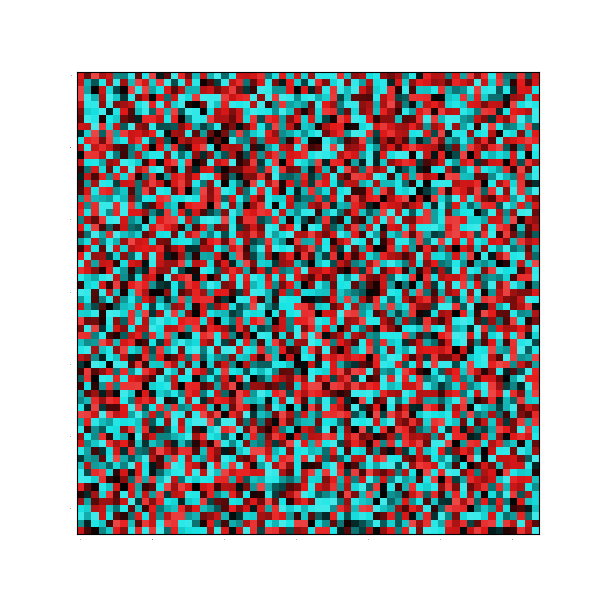
\includegraphics[width=0.20\textwidth]{imgs/0.png}}
      \subfigure[$\tau=0.5$]{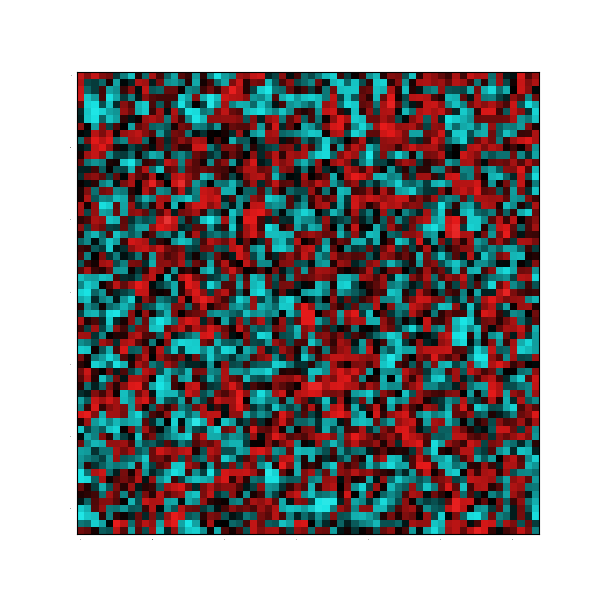
\includegraphics[width=0.20\textwidth]{imgs/0_5.png}}
      \subfigure[$\tau=2$]{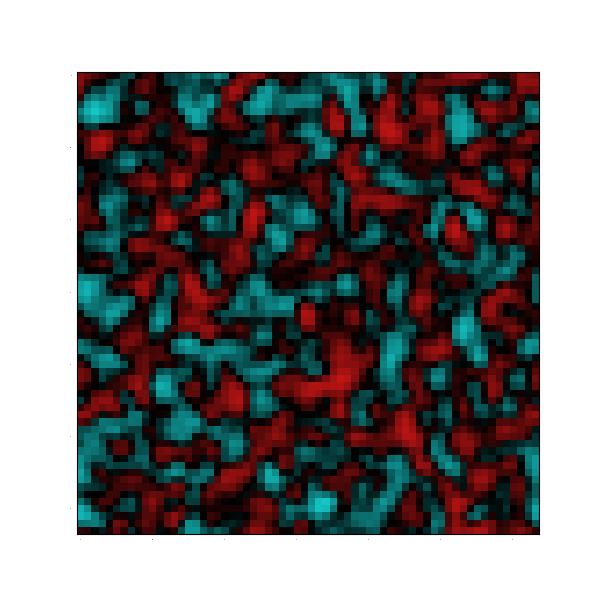
\includegraphics[width=0.20\textwidth]{imgs/2.png}} 
      \subfigure[$\tau=10$]{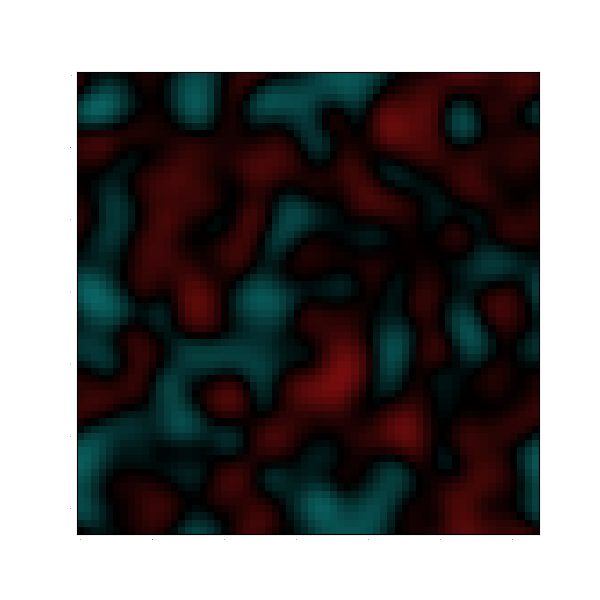
\includegraphics[width=0.20\textwidth]{imgs/10.png}}
          \caption{Effect of flow time evolution on a random lattice in the symmetric phase. Red and blue indicate positive and negative values of the field in 2D spacetime.}
  \label{fig:flow}
\end{figure}

\end{itemize}
\end{frame}

\begin{frame}
\frametitle{Non-Linear $\sigma$ Model}
\begin{itemize}
    \item a nonperturbative model in Quantum Field Theory which provides a good toy model for Quantum Chromodynamics
    \item characterized by the action
        \begin{equation*}
            S = \frac{1}{2g} \int d^2x \: \partial_\mu \vec{\phi}(x) \cdot \partial^\mu \vec{\phi}(x)
        \end{equation*}
    where the $\vec{\phi}(x)$ is a 3-component vector with norm 1 and $g$ is a coupling constant. 
\item Merits 
    \begin{itemize}
        \item mass gap
        \item asymptotic freedom
        \item $O(2)$ renormalizability
        \item in condensed matter, models Heisenberg ferromagnets
    \end{itemize}
\end{itemize}
\end{frame}

\begin{frame}
    \frametitle{Goals}
    \begin{itemize}
        \item Computationally implement the simpler $\phi^4$ theory to verify code.
        \item Transition to $O(3)$ nonlinear $\sigma$ model.
        \item Calculate twist-2 operators and vacuum expectation value with gradient flow applied.
        \item Other future paths:
            \begin{itemize}
                \item Consider topological charge
                \item Explore Wilson coefficients 
            \end{itemize}

    \end{itemize}
\end{frame}

\begin{frame}
    \frametitle{Broad Motivation}
    To understand Deep Inelastic Scattering (DIS)
    \begin{itemize}
        \item Twist-2 operators $\rightarrow$ Mellin moments $\rightarrow$ Parton Distribution Functions $\rightarrow$ DIS Cross Sections
    \end{itemize}
\end{frame}
%------------------------------------------------

\begin{frame}
    \frametitle{Computational Methods}
\begin{itemize}
    \item Use a Markov Chain Monte Carlo method to simulate lattice in 2D and 3D
        \begin{itemize}
            \item Metropolis algorithm to generate random changes
            \item Wolff cluster algorithm to remove metastable states
            \item Implement checkerboard algorithm to parallelize Metropolis algorithm
        \end{itemize}

    \item \textbf{By sampling the lattice at set intervals, we can calculate statical estimates of arbitrary operators.}
\end{itemize}

\end{frame}

\begin{frame}
    \frametitle{Markov Chain Monte Carlo}
\begin{enumerate}
    \item Start with random lattice (known as ``hot start'')
    \item Repeatedly transition from old configuration $\mu$ to new configuration $\nu$ with probability $P(\mu\rightarrow\nu)$.
    \item After a thermalization period, record observables at certain intervals. 
    \item Take the statistical mean
\end{enumerate}
\end{frame}

\begin{frame}
    \frametitle{Metropolis Algorithm}
    For each site, propose a new value and accept change with probability
        \begin{equation*}
    P(\mu\rightarrow\nu) = \begin{cases} 
        e^{-(S_\nu - S_\mu)} & S_\nu > S_\mu \\
        1 & \mathrm{S_\nu \leq S_\mu} \\
       \end{cases}
        \end{equation*} 
        A \textbf{sweep} consists of perfoming this on every site.

\end{frame}

\begin{frame}
    \frametitle{Wolff Cluster Algorithm}
        \textbf{Problem}: Markov Chain gets ``stuck'' in metastable states, i.e. local minima of the action.

        \textbf{Solution}: Identify cluster of similar-values points and flip the sign.
    \begin{enumerate}
        \item Recursively grow a cluster with the probability of adding a new site
        \begin{equation*}
            P_{add} = 1-e^{-2\phi_a\cdot\phi_b}.
        \end{equation*}
        \item Flip sign of sites
    

    \end{enumerate}
    \begin{figure}[h]

      \centering
          \subfigure[before]{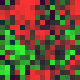
\includegraphics[width=0.20\textwidth]{imgs/wolff1}}
          \subfigure[after]{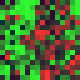
\includegraphics[width=0.20\textwidth]{imgs/wolff2}}
          \caption{Wolff cluster algorithm applied on $\phi^4$ lattice in $1+1$ dimensions, red corresponding to positive values and green to negative}
      \label{fig:flow}
    \end{figure}
\end{frame}

\begin{frame}
    \frametitle{Checkerboard Parallelization Algorithm}
    \begin{itemize}
        \item Split lattice into ``white'' and ``black'' sites. 
        \item Then, perform metropolis sweep on white sites in parallel, then black sites.
        \item Ensures independence of sweeps.
\end{itemize}

    \begin{figure}[h]

      \centering
          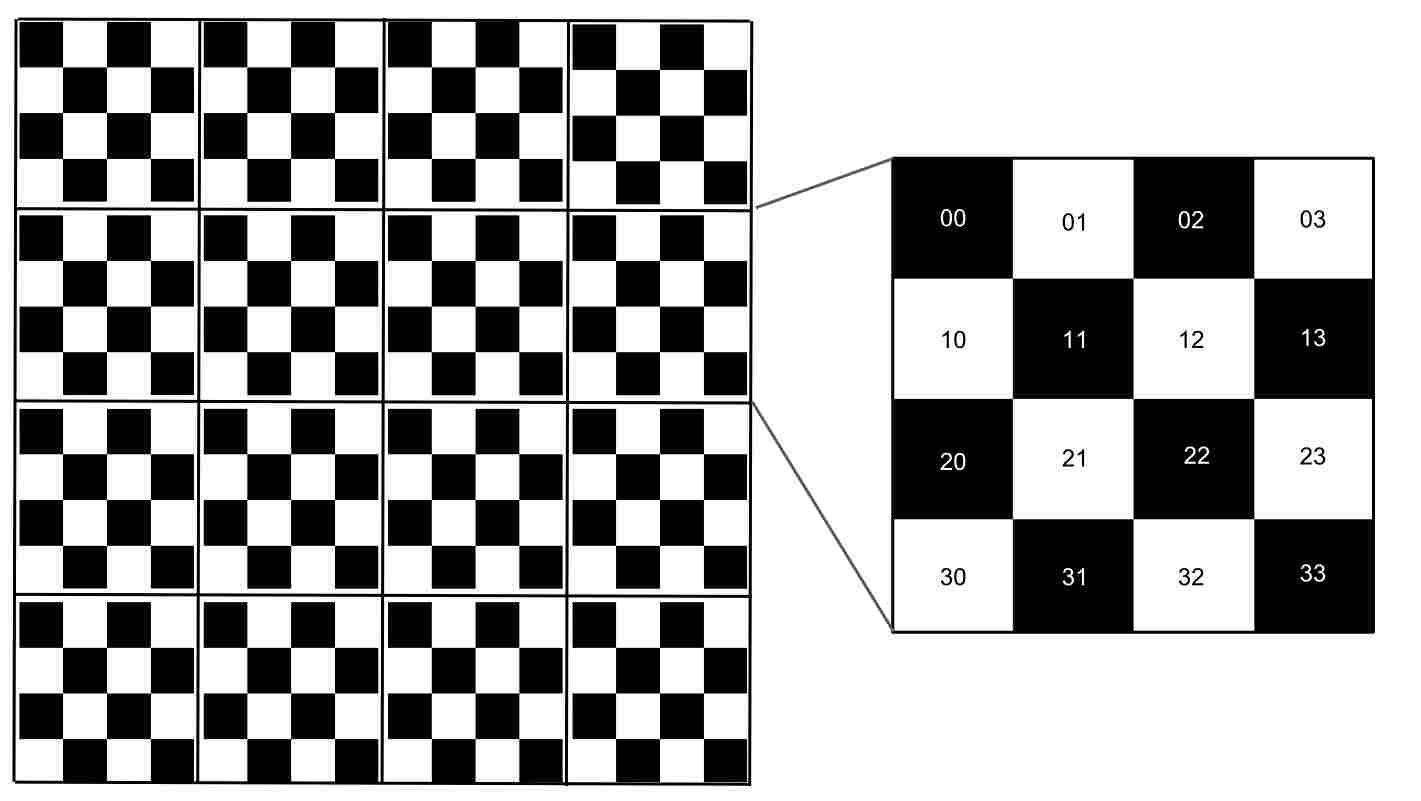
\includegraphics[width=0.5\textwidth]{imgs/checkerboard}
          \caption{Illustration of checkerboard algorithm\footnote{Yang, Kun, et al. "High performance Monte Carlo simulation of Ising model on TPU clusters." Proceedings of the International Conference for High Performance Computing, Networking, Storage and Analysis. 2019.}}
    \end{figure}

\end{frame}


\begin{frame}
    \frametitle{$\phi^4$ model}
    \begin{itemize}
        \item Given by the Euclidean action
            \begin{equation}
                S_E = \int d^D x \left[ \partial^\mu \phi \partial_\mu\phi + \frac{1}{2} m_0^2 \phi^2 + \frac{\lambda}{4}\phi^4\right]
            \end{equation} 

        \item Simplest interacting field
        \item In 1+1 dimensions, exhibits spontaneous symmetry breaking at critical $m_0^2$.


    \end{itemize}

    We measure\ldots
\begin{itemize}
    \item Magnetization: $\langle |\bar\phi|\rangle$
    \item Susceptibility: $\chi = \langle {\bar\phi}^2\rangle - \langle\bar\phi\rangle^2$
    \item Binder cumulant: $U = 1 - \frac{\langle {\bar\phi}^4\rangle}{3 \langle {\bar\phi}^2\rangle^2}$
\end{itemize}
\end{frame}

\begin{frame}
    \frametitle{Computational Implementation}
    \begin{enumerate}
        \item Begin with simple Python $\phi^4$ model with Cython for efficiency
        \item Transition to C++ code, generalized to nonlinear $\sigma$ model
        \item Compare results of Python and C++ code.
    \end{enumerate}
    \begin{block}{Parallelization}
        Message Passing Interface: shared RAM between processes.
    \end{block}
\end{frame}




\begin{frame}
\frametitle{Spontaneous Symmetry Breaking in $\phi^4$ model}
\begin{figure}[h]
  \centering
      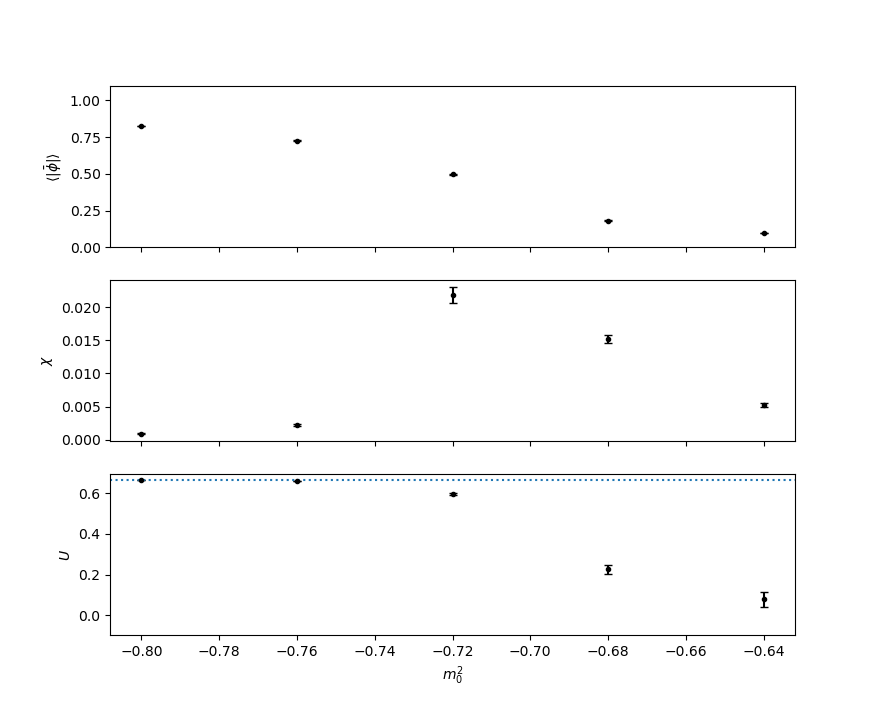
\includegraphics[width=0.7\textwidth]{imgs/phi4.png}
      \caption{Average $\bar\phi$, Binder cumulant and susceptibility for various $m_0^2$ values. $\lambda=0.5$, $L=64$, $1000$ measurements, $1000$ sweep thermalization with measurements taken every $100$ sweeps.}
  \label{fig:flow}
\end{figure}
\end{frame}


\begin{frame}
\frametitle{Comparison between Python and C++ code}
\begin{figure}[h]
  \centering
      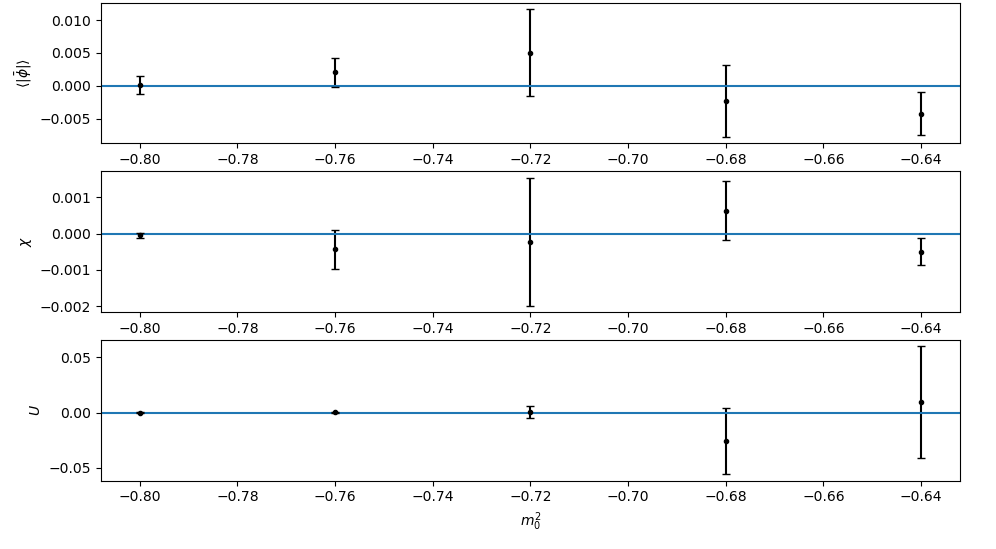
\includegraphics[width=0.9\textwidth]{imgs/compare.png}
      \caption{Absolute difference between Python and C++ results of average $\bar\phi$, Binder cumulant and susceptibility for various $m_0^2$ values. $\lambda=0.5$, $L=64$, $1000$ measurements, $1000$ sweep thermalization with measurements taken every $100$ sweeps. }

  \label{fig:flow}
\end{figure}
\end{frame}

\begin{frame}
\frametitle{Future Work}
\begin{itemize}
    \item Fully implement nonlinear $\sigma$ model.
    \item Calculate twist-2 operators and vacuum expectation value
    \item Expand to 3 dimensions
    \item Profile and optimize C++ code
    \item Mathematical analysis of results
\end{itemize}

\end{frame}

%%------------------------------------------------

%\begin{frame}
%\frametitle{Multiple Columns}
%\begin{columns}[c] % The "c" option specifies centered vertical alignment while the "t" option is used for top vertical alignment

%\column{.45\textwidth} % Left column and width
%\textbf{Heading}
%\begin{enumerate}
%\item Statement
%\item Explanation
%\item Example
%\end{enumerate}

%\column{.5\textwidth} % Right column and width
%Lorem ipsum dolor sit amet, consectetur adipiscing elit. Integer lectus nisl, ultricies in feugiat rutrum, porttitor sit amet augue. Aliquam ut tortor mauris. Sed volutpat ante purus, quis accumsan dolor.

%\end{columns}
%\end{frame}
%\begin{frame}
%\frametitle{Blocks of Highlighted Text}

%\begin{block}{Block 2}
%Pellentesque sed tellus purus. Class aptent taciti sociosqu ad litora torquent per conubia nostra, per inceptos himenaeos. Vestibulum quis magna at risus dictum tempor eu vitae velit.
%\end{block}

%\begin{block}{Block 3}
%Suspendisse tincidunt sagittis gravida. Curabitur condimentum, enim sed venenatis rutrum, ipsum neque consectetur orci, sed blandit justo nisi ac lacus.
%\end{block}
%\end{frame}

%%------------------------------------------------

%\begin{frame}
%\frametitle{Multiple Columns}
%\begin{columns}[c] % The "c" option specifies centered vertical alignment while the "t" option is used for top vertical alignment

%\column{.45\textwidth} % Left column and width
%\textbf{Heading}
%\begin{enumerate}
%\item Statement
%\item Explanation
%\item Example
%\end{enumerate}

%\column{.5\textwidth} % Right column and width
%Lorem ipsum dolor sit amet, consectetur adipiscing elit. Integer lectus nisl, ultricies in feugiat rutrum, porttitor sit amet augue. Aliquam ut tortor mauris. Sed volutpat ante purus, quis accumsan dolor.

%\end{columns}
%\end{frame}

%%------------------------------------------------
%\section{Second Section}
%%------------------------------------------------

%\begin{frame}
%\frametitle{Table}
%\begin{table}
%\begin{tabular}{l l l}
%\toprule
%\textbf{Treatments} & \textbf{Response 1} & \textbf{Response 2}\\
%\midrule
%Treatment 1 & 0.0003262 & 0.562 \\
%Treatment 2 & 0.0015681 & 0.910 \\
%Treatment 3 & 0.0009271 & 0.296 \\
%\bottomrule
%\end{tabular}
%\caption{Table caption}
%\end{table}
%\end{frame}

%%------------------------------------------------

%\begin{frame}
%\frametitle{Theorem}
%\begin{theorem}[Mass--energy equivalence]
%$E = mc^2$
%\end{theorem}
%\end{frame}

%%------------------------------------------------

%\begin{frame}[fragile] % Need to use the fragile option when verbatim is used in the slide
%\frametitle{Verbatim}
%\begin{example}[Theorem Slide Code]
%\begin{verbatim}
%\begin{frame}
%\frametitle{Theorem}
%\begin{theorem}[Mass--energy equivalence]
%$E = mc^2$
%\end{theorem}
%\end{frame}\end{verbatim}
%\end{example}
%\end{frame}

%%------------------------------------------------

%\begin{frame}
%\frametitle{Figure}
%Uncomment the code on this slide to include your own image from the same directory as the template .TeX file.
%%\begin{figure}
%%\includegraphics[width=0.8\linewidth]{test}
%%\end{figure}
%\end{frame}

%%------------------------------------------------

%\begin{frame}[fragile] % Need to use the fragile option when verbatim is used in the slide
%\frametitle{Citation}
%An example of the \verb|\cite| command to cite within the presentation:\\~

%This statement requires citation \cite{p1}.
%\end{frame}

%%------------------------------------------------

%\begin{frame}
%\frametitle{References}
%\footnotesize{
%\begin{thebibliography}{99} % Beamer does not support BibTeX so references must be inserted manually as below
%\bibitem[Smith, 2012]{p1} John Smith (2012)
%\newblock Title of the publication
%\newblock \emph{Journal Name} 12(3), 45 -- 678.
%\end{thebibliography}
%}
%\end{frame}

%%------------------------------------------------

%\begin{frame}
%\Huge{\centerline{The End}}
%\end{frame}

%%----------------------------------------------------------------------------------------

\end{document} 
